\documentclass[]{book}
\usepackage{lmodern}
\usepackage{amssymb,amsmath}
\usepackage{ifxetex,ifluatex}
\usepackage{fixltx2e} % provides \textsubscript
\ifnum 0\ifxetex 1\fi\ifluatex 1\fi=0 % if pdftex
  \usepackage[T1]{fontenc}
  \usepackage[utf8]{inputenc}
\else % if luatex or xelatex
  \ifxetex
    \usepackage{mathspec}
  \else
    \usepackage{fontspec}
  \fi
  \defaultfontfeatures{Ligatures=TeX,Scale=MatchLowercase}
\fi
% use upquote if available, for straight quotes in verbatim environments
\IfFileExists{upquote.sty}{\usepackage{upquote}}{}
% use microtype if available
\IfFileExists{microtype.sty}{%
\usepackage{microtype}
\UseMicrotypeSet[protrusion]{basicmath} % disable protrusion for tt fonts
}{}
\usepackage[margin=1in]{geometry}
\usepackage{hyperref}
\hypersetup{unicode=true,
            pdftitle={OCD-NET \& BDD-NET therapist resources},
            pdfauthor={Oskar Flygare, Christian Rück, Jesper Enander \& Erik Andersson},
            pdfborder={0 0 0},
            breaklinks=true}
\urlstyle{same}  % don't use monospace font for urls
\usepackage{natbib}
\bibliographystyle{apalike}
\usepackage{longtable,booktabs}
\usepackage{graphicx,grffile}
\makeatletter
\def\maxwidth{\ifdim\Gin@nat@width>\linewidth\linewidth\else\Gin@nat@width\fi}
\def\maxheight{\ifdim\Gin@nat@height>\textheight\textheight\else\Gin@nat@height\fi}
\makeatother
% Scale images if necessary, so that they will not overflow the page
% margins by default, and it is still possible to overwrite the defaults
% using explicit options in \includegraphics[width, height, ...]{}
\setkeys{Gin}{width=\maxwidth,height=\maxheight,keepaspectratio}
\IfFileExists{parskip.sty}{%
\usepackage{parskip}
}{% else
\setlength{\parindent}{0pt}
\setlength{\parskip}{6pt plus 2pt minus 1pt}
}
\setlength{\emergencystretch}{3em}  % prevent overfull lines
\providecommand{\tightlist}{%
  \setlength{\itemsep}{0pt}\setlength{\parskip}{0pt}}
\setcounter{secnumdepth}{5}
% Redefines (sub)paragraphs to behave more like sections
\ifx\paragraph\undefined\else
\let\oldparagraph\paragraph
\renewcommand{\paragraph}[1]{\oldparagraph{#1}\mbox{}}
\fi
\ifx\subparagraph\undefined\else
\let\oldsubparagraph\subparagraph
\renewcommand{\subparagraph}[1]{\oldsubparagraph{#1}\mbox{}}
\fi

%%% Use protect on footnotes to avoid problems with footnotes in titles
\let\rmarkdownfootnote\footnote%
\def\footnote{\protect\rmarkdownfootnote}

%%% Change title format to be more compact
\usepackage{titling}

% Create subtitle command for use in maketitle
\newcommand{\subtitle}[1]{
  \posttitle{
    \begin{center}\large#1\end{center}
    }
}

\setlength{\droptitle}{-2em}

  \title{OCD-NET \& BDD-NET therapist resources}
    \pretitle{\vspace{\droptitle}\centering\huge}
  \posttitle{\par}
    \author{Oskar Flygare, Christian Rück, Jesper Enander \& Erik Andersson}
    \preauthor{\centering\large\emph}
  \postauthor{\par}
      \predate{\centering\large\emph}
  \postdate{\par}
    \date{2018-11-13}

\usepackage{booktabs}
\usepackage{amsthm}
\makeatletter
\def\thm@space@setup{%
  \thm@preskip=8pt plus 2pt minus 4pt
  \thm@postskip=\thm@preskip
}
\makeatother

\usepackage{amsthm}
\newtheorem{theorem}{Theorem}[chapter]
\newtheorem{lemma}{Lemma}[chapter]
\theoremstyle{definition}
\newtheorem{definition}{Definition}[chapter]
\newtheorem{corollary}{Corollary}[chapter]
\newtheorem{proposition}{Proposition}[chapter]
\theoremstyle{definition}
\newtheorem{example}{Example}[chapter]
\theoremstyle{definition}
\newtheorem{exercise}{Exercise}[chapter]
\theoremstyle{remark}
\newtheorem*{remark}{Remark}
\newtheorem*{solution}{Solution}
\begin{document}
\maketitle

{
\setcounter{tocdepth}{1}
\tableofcontents
}
\hypertarget{introduction}{%
\chapter{Introduction}\label{introduction}}

Welcome to our online therapist resource for the \emph{Web-CBT} platform
for \emph{OCD-NET} and \emph{BDD-NET}. We strive to continuously update
and improve this material and would appreciate any feedback. You can
reach us at
\href{mailto:ocdnet.support@webcbt.se}{\nolinkurl{ocdnet.support@webcbt.se}}
or talk to us in person at a training session.

\hypertarget{description-of-ocd-net-and-bdd-net}{%
\section{Description of OCD-NET and
BDD-NET}\label{description-of-ocd-net-and-bdd-net}}

OCD-NET and BDD-NET are therapist-guided internet-based cognitive
behaviour (ICBT) therapies for OCD and BDD, respectively. In ICBT,
patients have an identified therapist providing support and feedback
throughout treatment. All contact with the therapist occurs through the
treatment platform as asynchronous text messages (like e-mail or SMS).

\hypertarget{type-of-treatment}{%
\section{Type of treatment}\label{type-of-treatment}}

The intended use of OCD-NET and BDD-NET are within a stepped care model
as an alternative to brief individual CBT, group CBT, serotonin reuptake
inhibitors (SSRIs), or higher-intensity CBT for adults with mild to
moderate symptoms. The treatments are expected to be cost-saving
compared to individual CBT (10 hours or more intensive treatment) but
not compared to group CBT. Crucially, ICBT therapies typically require
less therapist time per patient (10-20 minutes per patient each week)
and could therefore release therapist time compared to individual CBT or
group CBT.

\hypertarget{background}{%
\section{Background}\label{background}}

Both OCD-NET and BDD-NET were initially developed by researchers at
Karolinska Institutet in Stockholm, Sweden. OCD-NET has been evaluated
in six clinical trials to date with results indicating that it is as
effective as regular face-to-face CBT, while requiring less therapist
time per patient and with the advantage of being accessible from any
device connected to the internet
\citep{andersson2011a, andersson2012, andersson2014a, andersson2015a, ruck2018}.
Similarly, BDD-NET has been evaluated in two clinical trials with
comparable results \citep{enander2014, enander2016}. Both treatments
were initially developed in Swedish but have been translated to English
and evaluated in pilot studies in New York (OCD-NET) and an
international pilot study (BDD-NET) \citep{patel2017}. \textless{}-
\textbf{ADD BDD GLOBAL}

\hypertarget{tasks-for-kristin}{%
\section{Tasks for Kristin}\label{tasks-for-kristin}}

\textbf{As therapist:}

\begin{itemize}
\tightlist
\item
  Log in as therapist 1
\item
  Write a message to patient 1
\item
  Review homework module 3 for patient 1
\item
  Remove a suicidality flag and comment ``Suicide risk assessment
  completed via telephone. Low risk'' for patient 1
\end{itemize}

\textbf{As patient:}

\begin{itemize}
\tightlist
\item
  Log in as patient 1
\item
  Answer questionnaires if they appear
\item
  Complete homework for module 4 (you can write whatever)
\item
  Write a message to the therapist
\end{itemize}

\hypertarget{using-the-technology}{%
\chapter{Using the technology}\label{using-the-technology}}

\hypertarget{quick-start}{%
\section{Quick start}\label{quick-start}}

If you want to explore the platform yourself, you can use test therapist
and test patient logins provided to try out the features (separate
document). We generally recommend that you use the platform while
reading this manual, to test features as you go along.

\hypertarget{platform-use-overview}{%
\section{Platform use overview}\label{platform-use-overview}}

There are five common scenarios during the course of treatment:

\begin{itemize}
\tightlist
\item
  Responding to messages
\item
  Reviewing homework
\item
  Opening new treatment modules
\item
  Reviewing questionnaires
\item
  Responding to warning flags
\end{itemize}

These actions can all be accessed in the participant overview, shown
below: 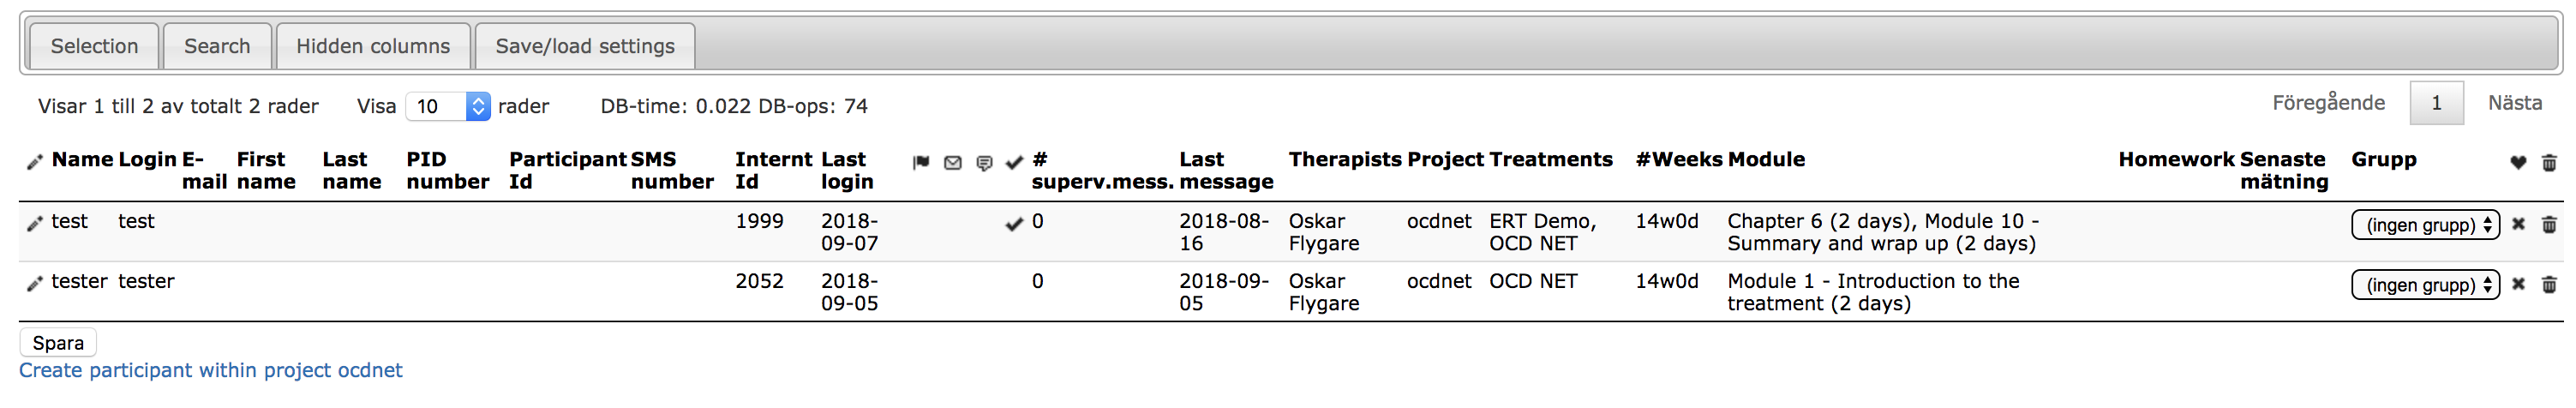
\includegraphics{images/participant-overview.png}

A typical day as a therapist includes responding to one or more
messages, reviewing homework and opening up a new module. Once in a
while therapists contact inactive patients or assess a warning flag.

\textbf{Quick note: We use Participant and Patient as synonyms here.}

\hypertarget{navigation}{%
\section{Navigation}\label{navigation}}

The majority of day to day tasks are accessed via the \emph{Participant
search} menu. The menu is located at the left-hand side of the browser
window, and clicking \emph{Participant search} will get you back to the
participant overview. To access individual participants, click the
pencil next to their name.

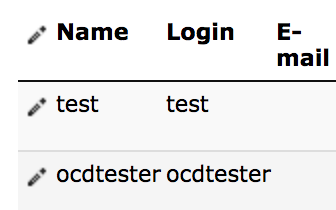
\includegraphics{images/pencil.png}

This menu may expand depending on administrative rights. Other parts of
the menu include administrative settings such as editing treatment
content, editing assessments, changing the way flags appear, and
changing settings to the site itself. These will not be relevant to most
therapists and we do not cover them in detail here. Just remember that
you can always go back to the default view by navigating to
\emph{Participant search} in the left-hand menu.

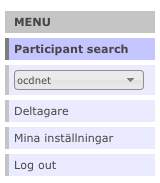
\includegraphics{images/therapist-menu.png}

\hypertarget{filtering-the-participant-overview}{%
\section{Filtering the participant
overview}\label{filtering-the-participant-overview}}

To get a quick overview of a long participant list, filter patients that
meet certain criteria, for example belonging to certain groups in
treatment of certain treatments. There is a button called
\emph{Selection} above the participant list. We recommend that
therapists use the ``My participants'' filter to show only patients
assigned to them.

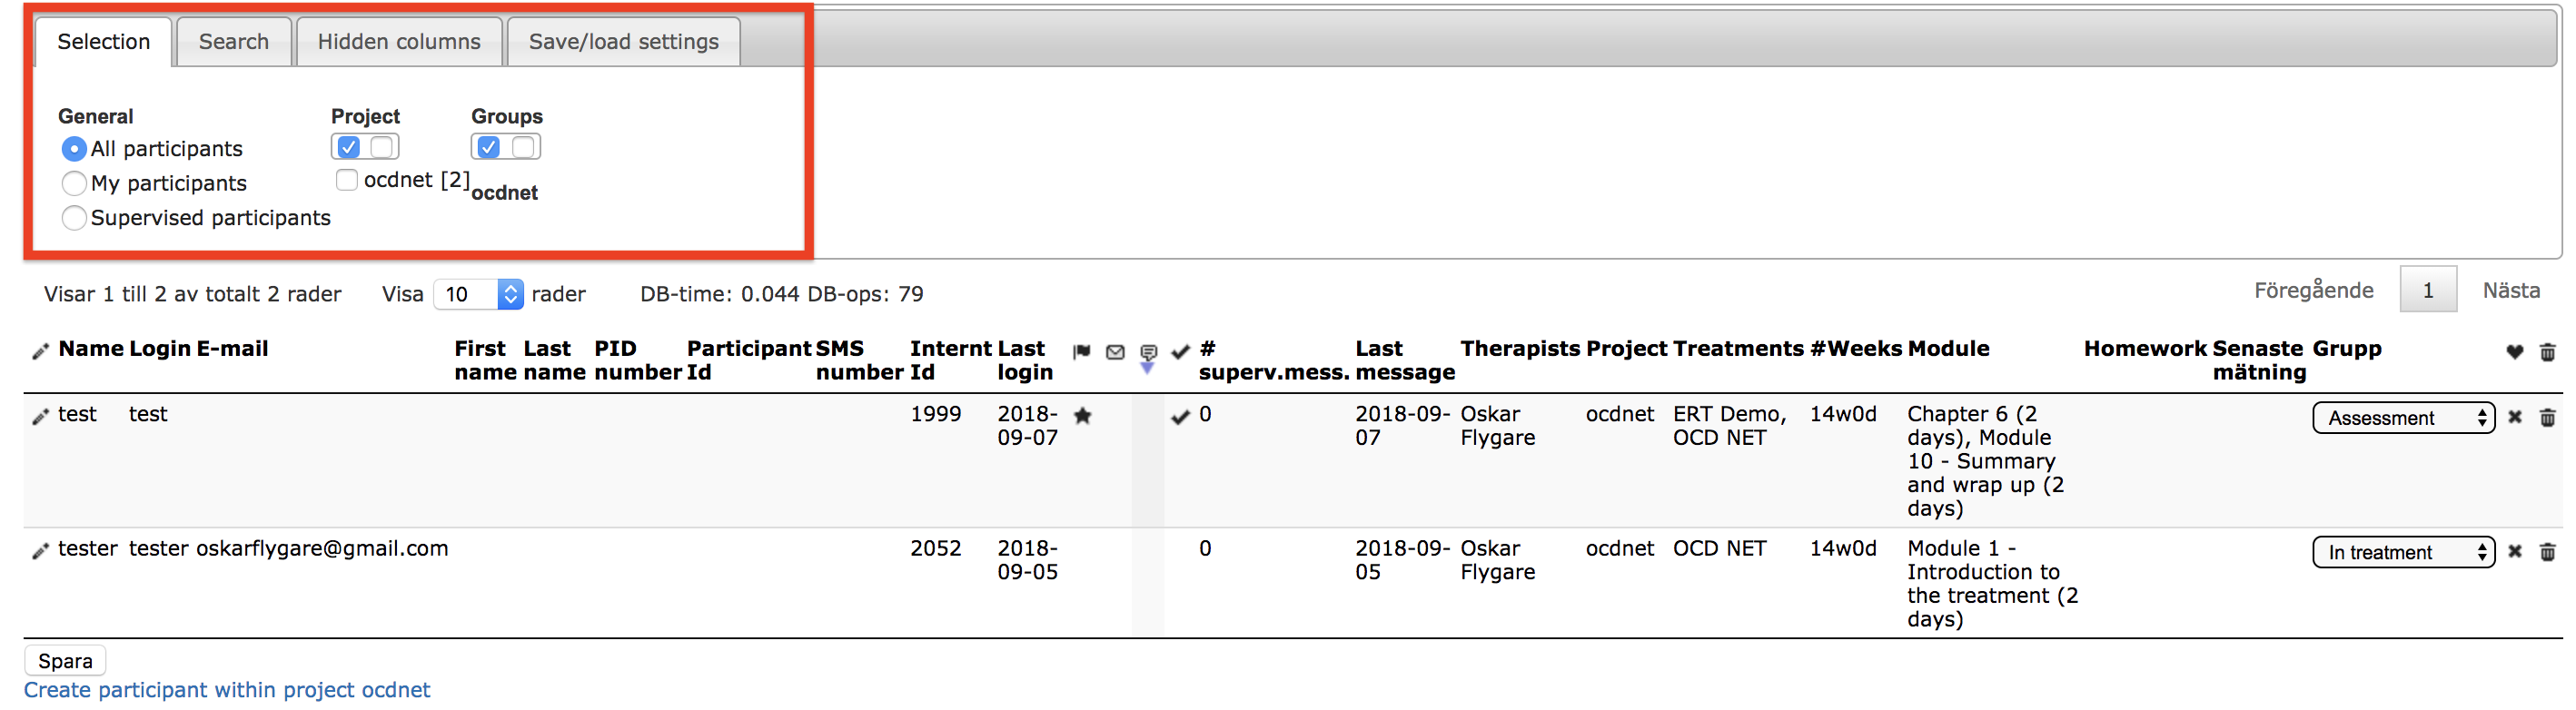
\includegraphics{images/filter-participants.png}

\hypertarget{writing-and-responding-to-messages}{%
\section{Writing and responding to
messages}\label{writing-and-responding-to-messages}}

A new message from a patient will be indicated by this icon turning red

\includegraphics{images/message-icon.png}. Navigate to \emph{Treatments
-\textgreater{} participant messages} to view the message and write a
response. See the chapter \emph{Being an effective ICBT therapist} for
guidelines on how to write messages.

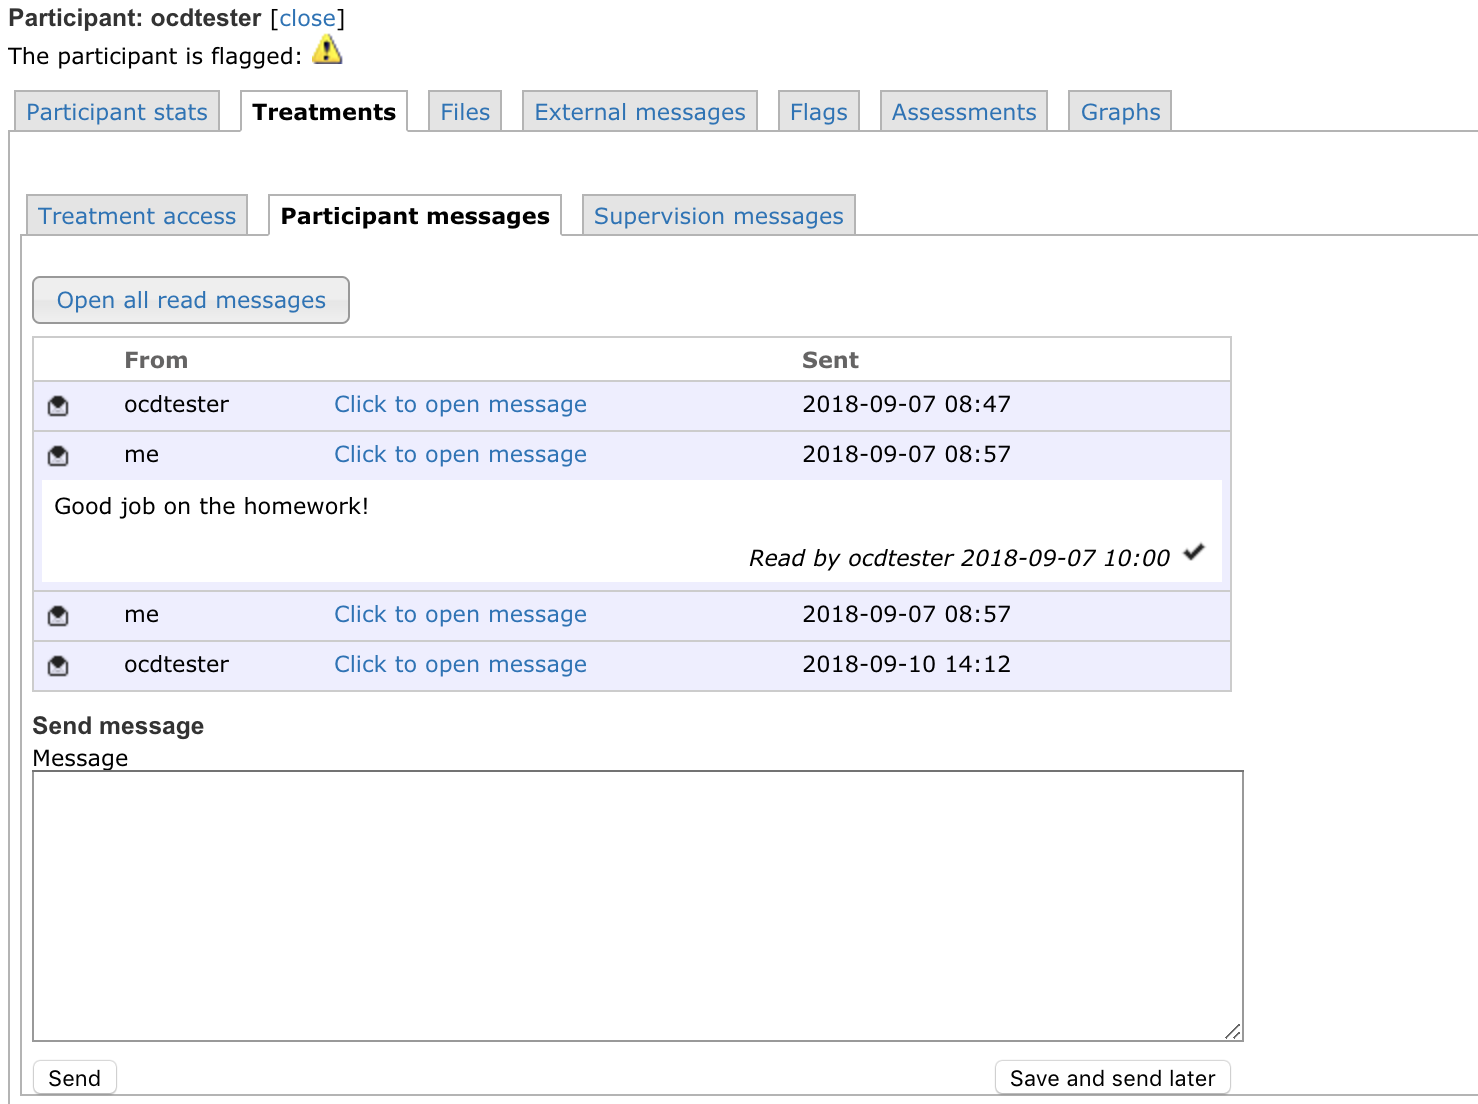
\includegraphics{images/therapist-messages.png}

\hypertarget{homework-review}{%
\section{Homework review}\label{homework-review}}

A completed homework assignment is shown in the \textbf{Homework} column
in the participant overview. Click the pencil next to the participant
and navigate to \emph{Treatments -\textgreater{} Treatment access} to
review the homework and mark it as completed.

\begin{figure}
\centering
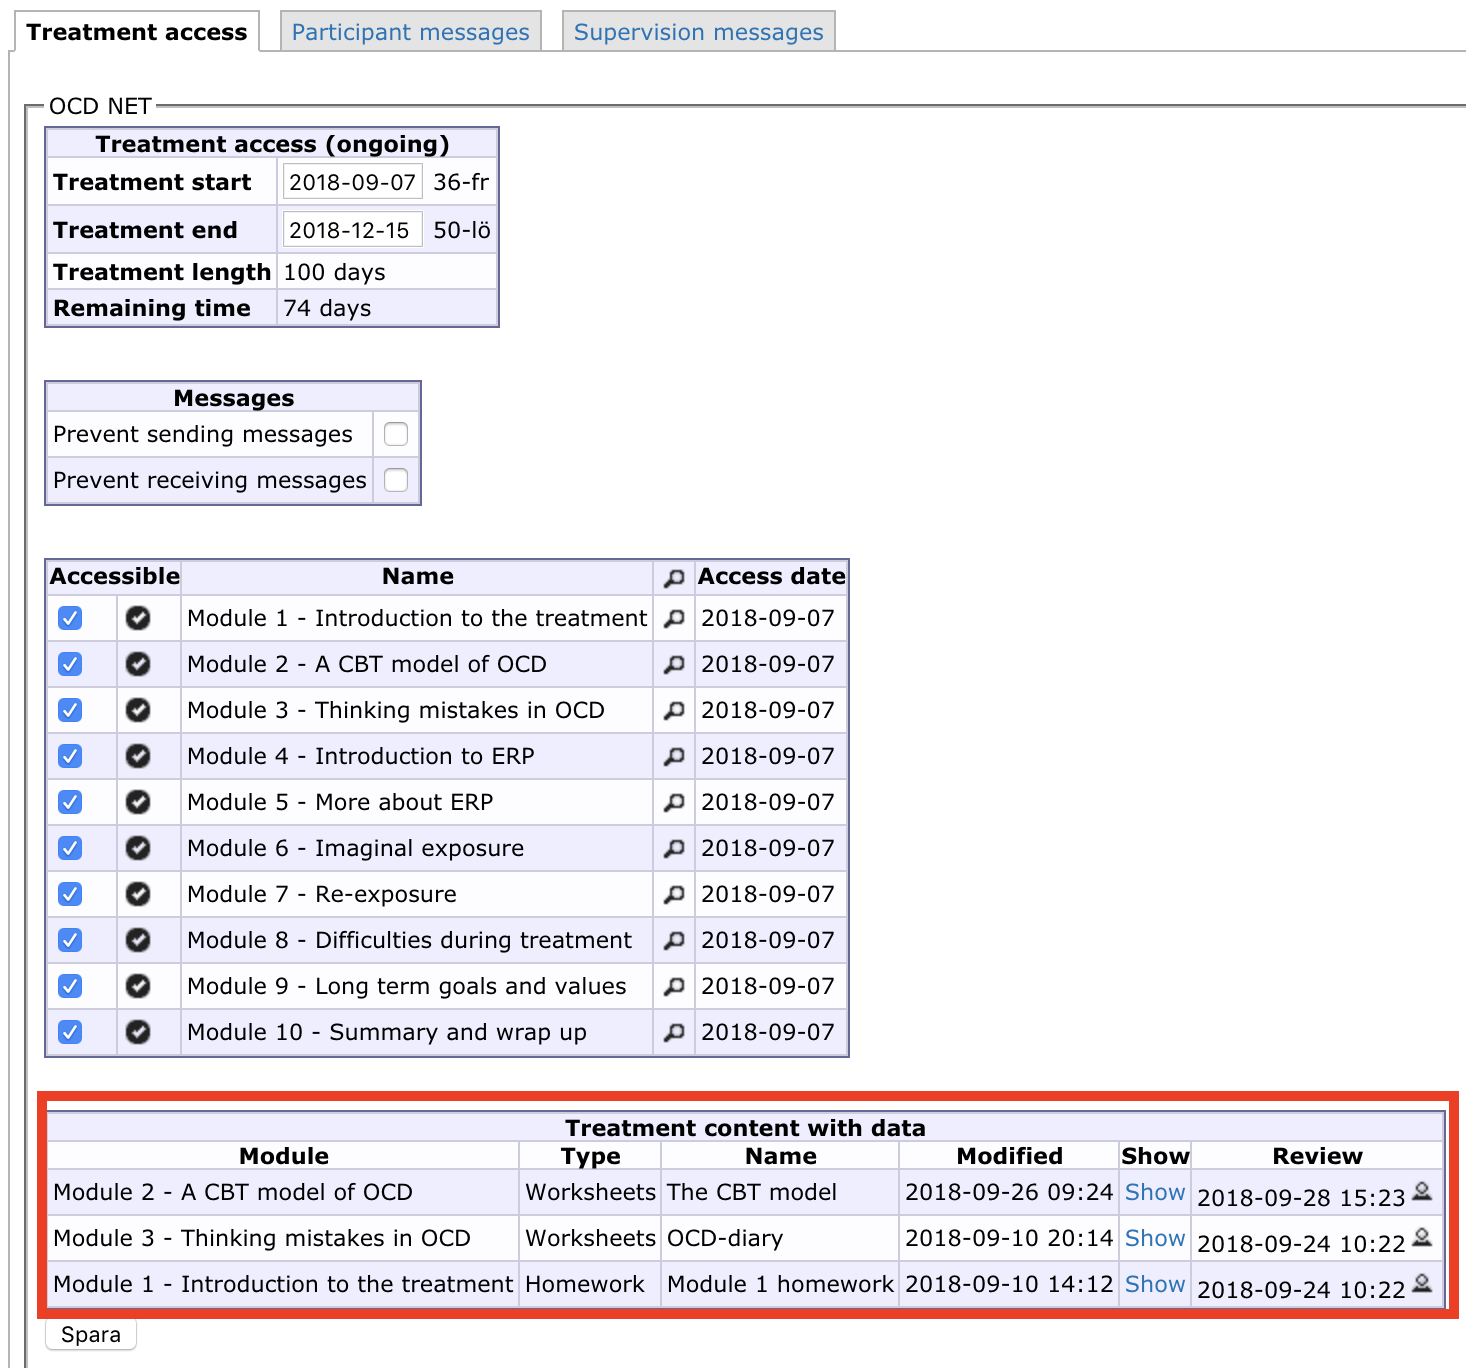
\includegraphics{images/homework-complete.png}
\caption{Completed homework assignments will show up for review in the
treatment overview}
\end{figure}

Internet-based CBT relies heavily on self-directed activities and
homework review is a good time to check whether the patient has grasped
important concepts and are able to apply them to their own situation.

\hypertarget{treatment-modules}{%
\section{Treatment modules}\label{treatment-modules}}

When a patient has read a module and completed the corresponding
homework assignment(s), they are ready for the next module. To grant
access to a new module, navigate to \emph{Treatments -\textgreater{}
Treatment access} and check the box next to the next module. A date will
appear next to the module indicating when the module was activated.
Patients automatically get a text message when they get access to a new
module.

\begin{figure}
\centering
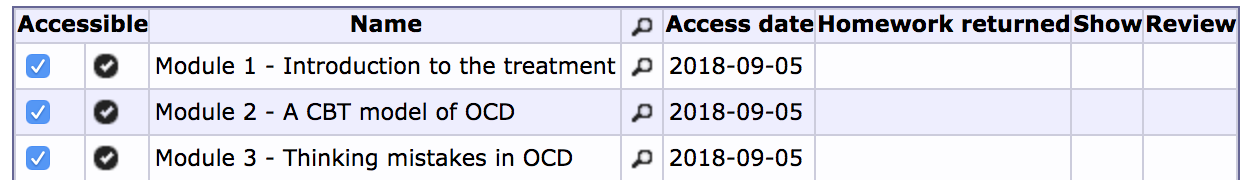
\includegraphics{images/module-access.png}
\caption{Check the box to the left to open a new module}
\end{figure}

The number of modules and weeks in treatment varies between treatment
protocols but a rough guideline is that patients should progress through
one module per week. Some treatment techniques, like exposure with
response prevention, are spread out across several modules to emphasise
their importance and give participants sufficient time to get started on
the technique.

\hypertarget{questionnaires}{%
\section{Questionnaires}\label{questionnaires}}

Before, during, and after treatment, patients are asked to fill out
questionnaires. When new questionnaires are activated they appear as the
patient logs onto the platform. Therapists can review and change which
questionnaires should appear at which day in \emph{Assessments} but we
recommend that therapists stick to the standard schedule whenever
possible.

\begin{figure}
\centering
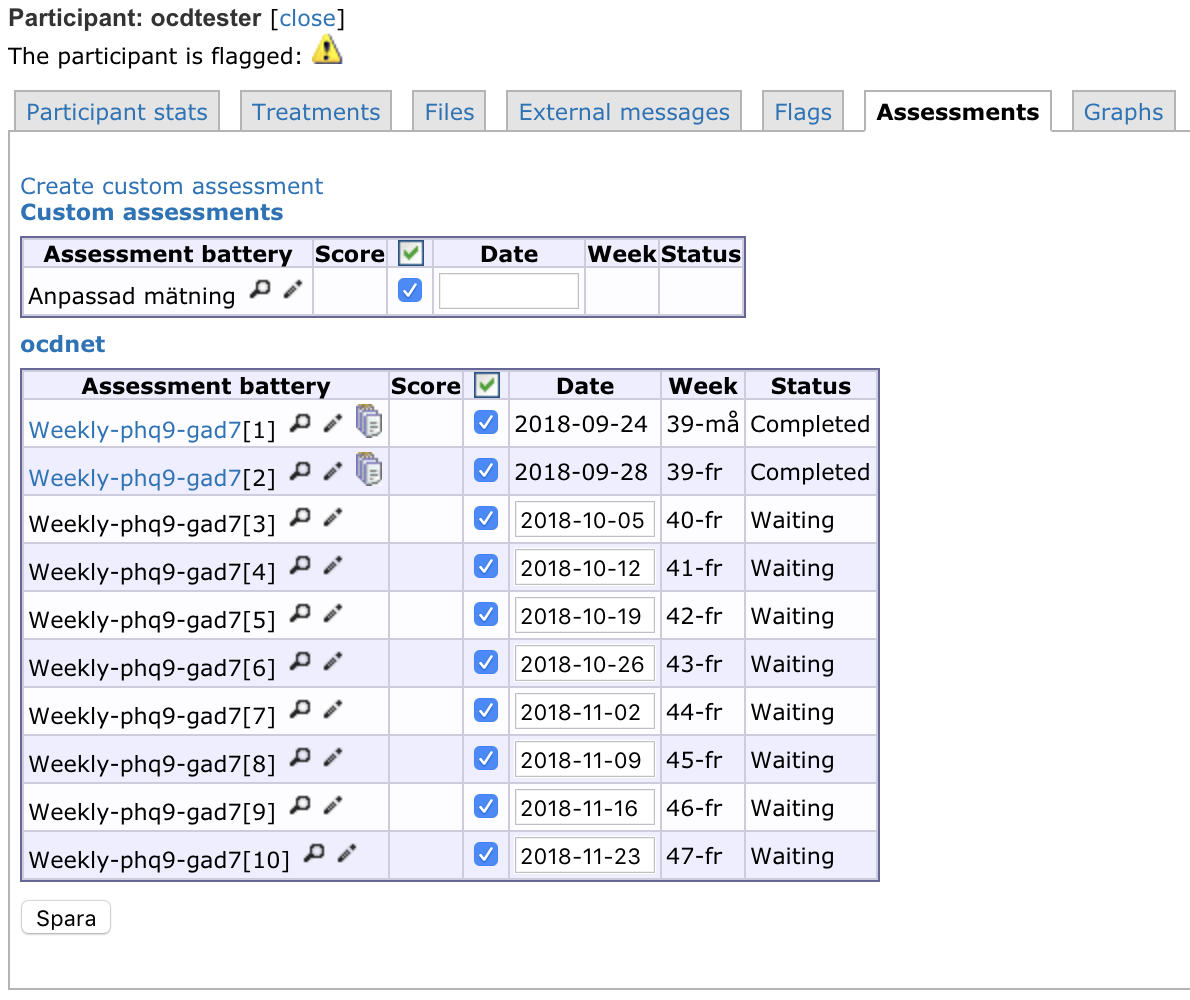
\includegraphics{images/assessments-list.png}
\caption{Questionnaires for each patient are listed in this view}
\end{figure}

\hypertarget{warning-flags}{%
\section{Warning flags}\label{warning-flags}}

The ICBT platform will display a \emph{warning flag} next to a patient's
name for certain events. The most common flags are due to inactivity or
non-response to questionnaires. These serve as prompts to therapists to
take further action, for example reaching out by phone to a patient or
sending them another text message reminder.

Once a warning flag has been noticed and dealt with, indicate the action
taken in the \emph{temporary flag text} box in the \emph{Participant
stats} tab (shown below). Please note, however that inactivity flags
automatically disappear once then patient uses the platform again.

\begin{figure}
\centering
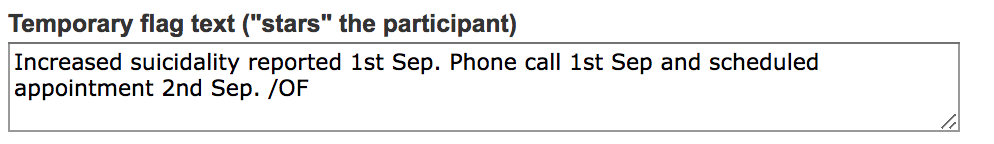
\includegraphics{images/temporary-flag-text.png}
\caption{Temporary flag texts aid communication between therapists when
they manage flags}
\end{figure}

\hypertarget{common-warning-flags}{%
\subsection{Common warning flags}\label{common-warning-flags}}

\begin{itemize}
\tightlist
\item
  Patient has not logged in for 7 days:
  
\includegraphics{images/login-inactivity-flag.png}
\item
  Patient has not written a message in 7 days:
  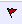
\includegraphics{images/message-inactivity-flag.png}
\item
  Patient has not responded to measurement in time:
  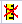
\includegraphics{images/measurement-delay-flag.png}
\item
  Patient has no assigned therapist:
  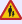
\includegraphics{images/notherapist-flag.png}
\item
  Treatment ends within 1 week:
  
\includegraphics{images/oneweek-therapyends-flag.png}
\item
  Treatment has ended: 
\includegraphics{images/therapy-ended-flag.png}
\end{itemize}

\hypertarget{suicidality-warning-flags}{%
\subsection{Suicidality warning flags}\label{suicidality-warning-flags}}

The most important type of warning flag is due to heightened
suicidality. The platform is configured to display this flag if a
patient responds 2 or 3 on the suicidality question in PHQ-9.

\begin{itemize}
\tightlist
\item
  Warning flag to indicate suicidal ideation:
  
\includegraphics{images/suicidality-warning.png}
\end{itemize}

\emph{Local clinical guidelines may overrule the general course of
action outlined here.}

\begin{enumerate}
\def\labelenumi{\arabic{enumi}.}
\tightlist
\item
  Call the patient immediately
\item
  Explain that it is standard procedure to call when a patient indicates
  heightened suicidal ideation
\item
  Follow a hierarchy of questions, such as M.I.N.I. interview, to assess
  level of suicidality
\item
  If the immediate risk is low (i.e.~PHQ-9 score of 2), make an
  agreement to check back in with the patient in a few days and give
  them contact information to the nearest 24-hour psychiatric care unit
\item
  If the immediate risk is high (i.e.~PHQ-9 score of 3), advise the
  patient to seek immediate help at your centre or at a 24-hour
  psychiatric care unit.
\end{enumerate}

Once the level of suicidality is deemed to be low enough to not require
further attention, therapists can remove the warning flag under the
\emph{Flags} tab for the participant.

\begin{figure}
\centering
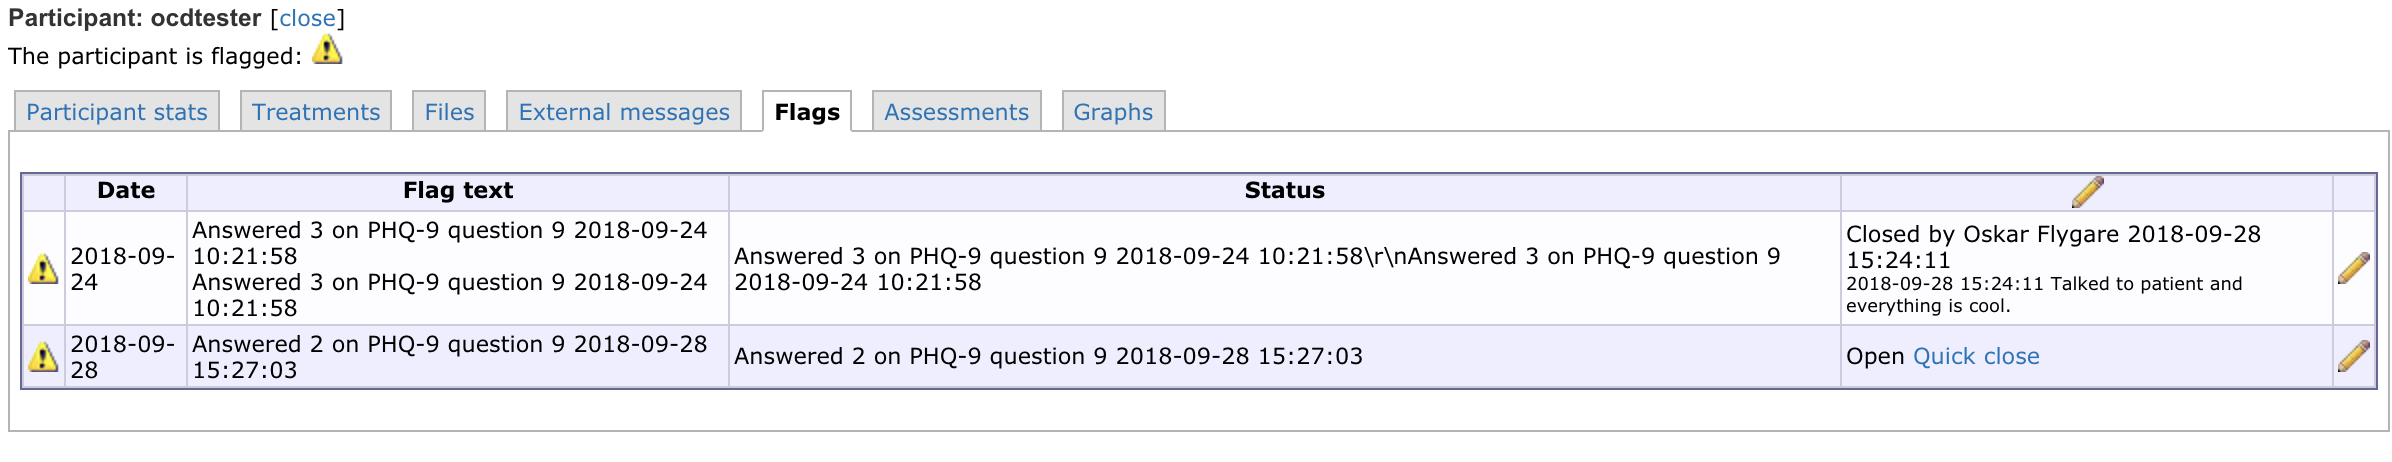
\includegraphics{images/flags-tab.png}
\caption{Flags are listed under the Flags tab, click on the pencil to
edit flag.}
\end{figure}

\begin{figure}
\centering
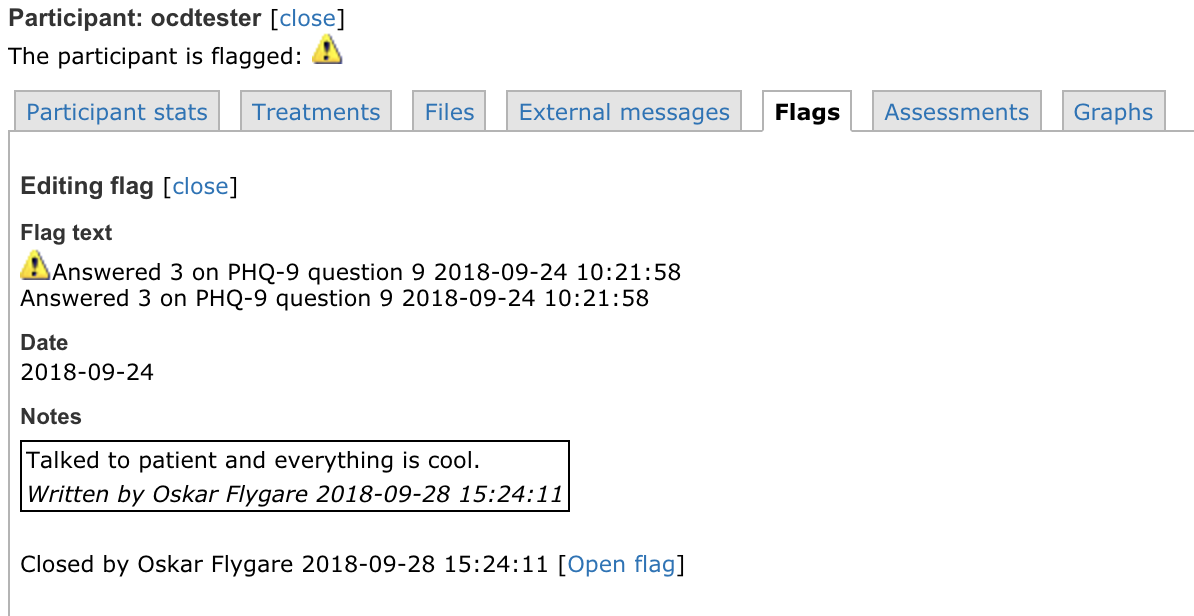
\includegraphics{images/remove-flag.png}
\caption{Once you have managed a flag, you can make a note that lists
actions taken, and remove the flag.}
\end{figure}

\hypertarget{supervision}{%
\section{Supervision}\label{supervision}}

Supervision through the platform makes it easy to connect feedback from
the supervisor to specific therapist messages and actions. The
supervision page is found at \emph{Treatment -\textgreater{} Supervision
messages} for each participant.

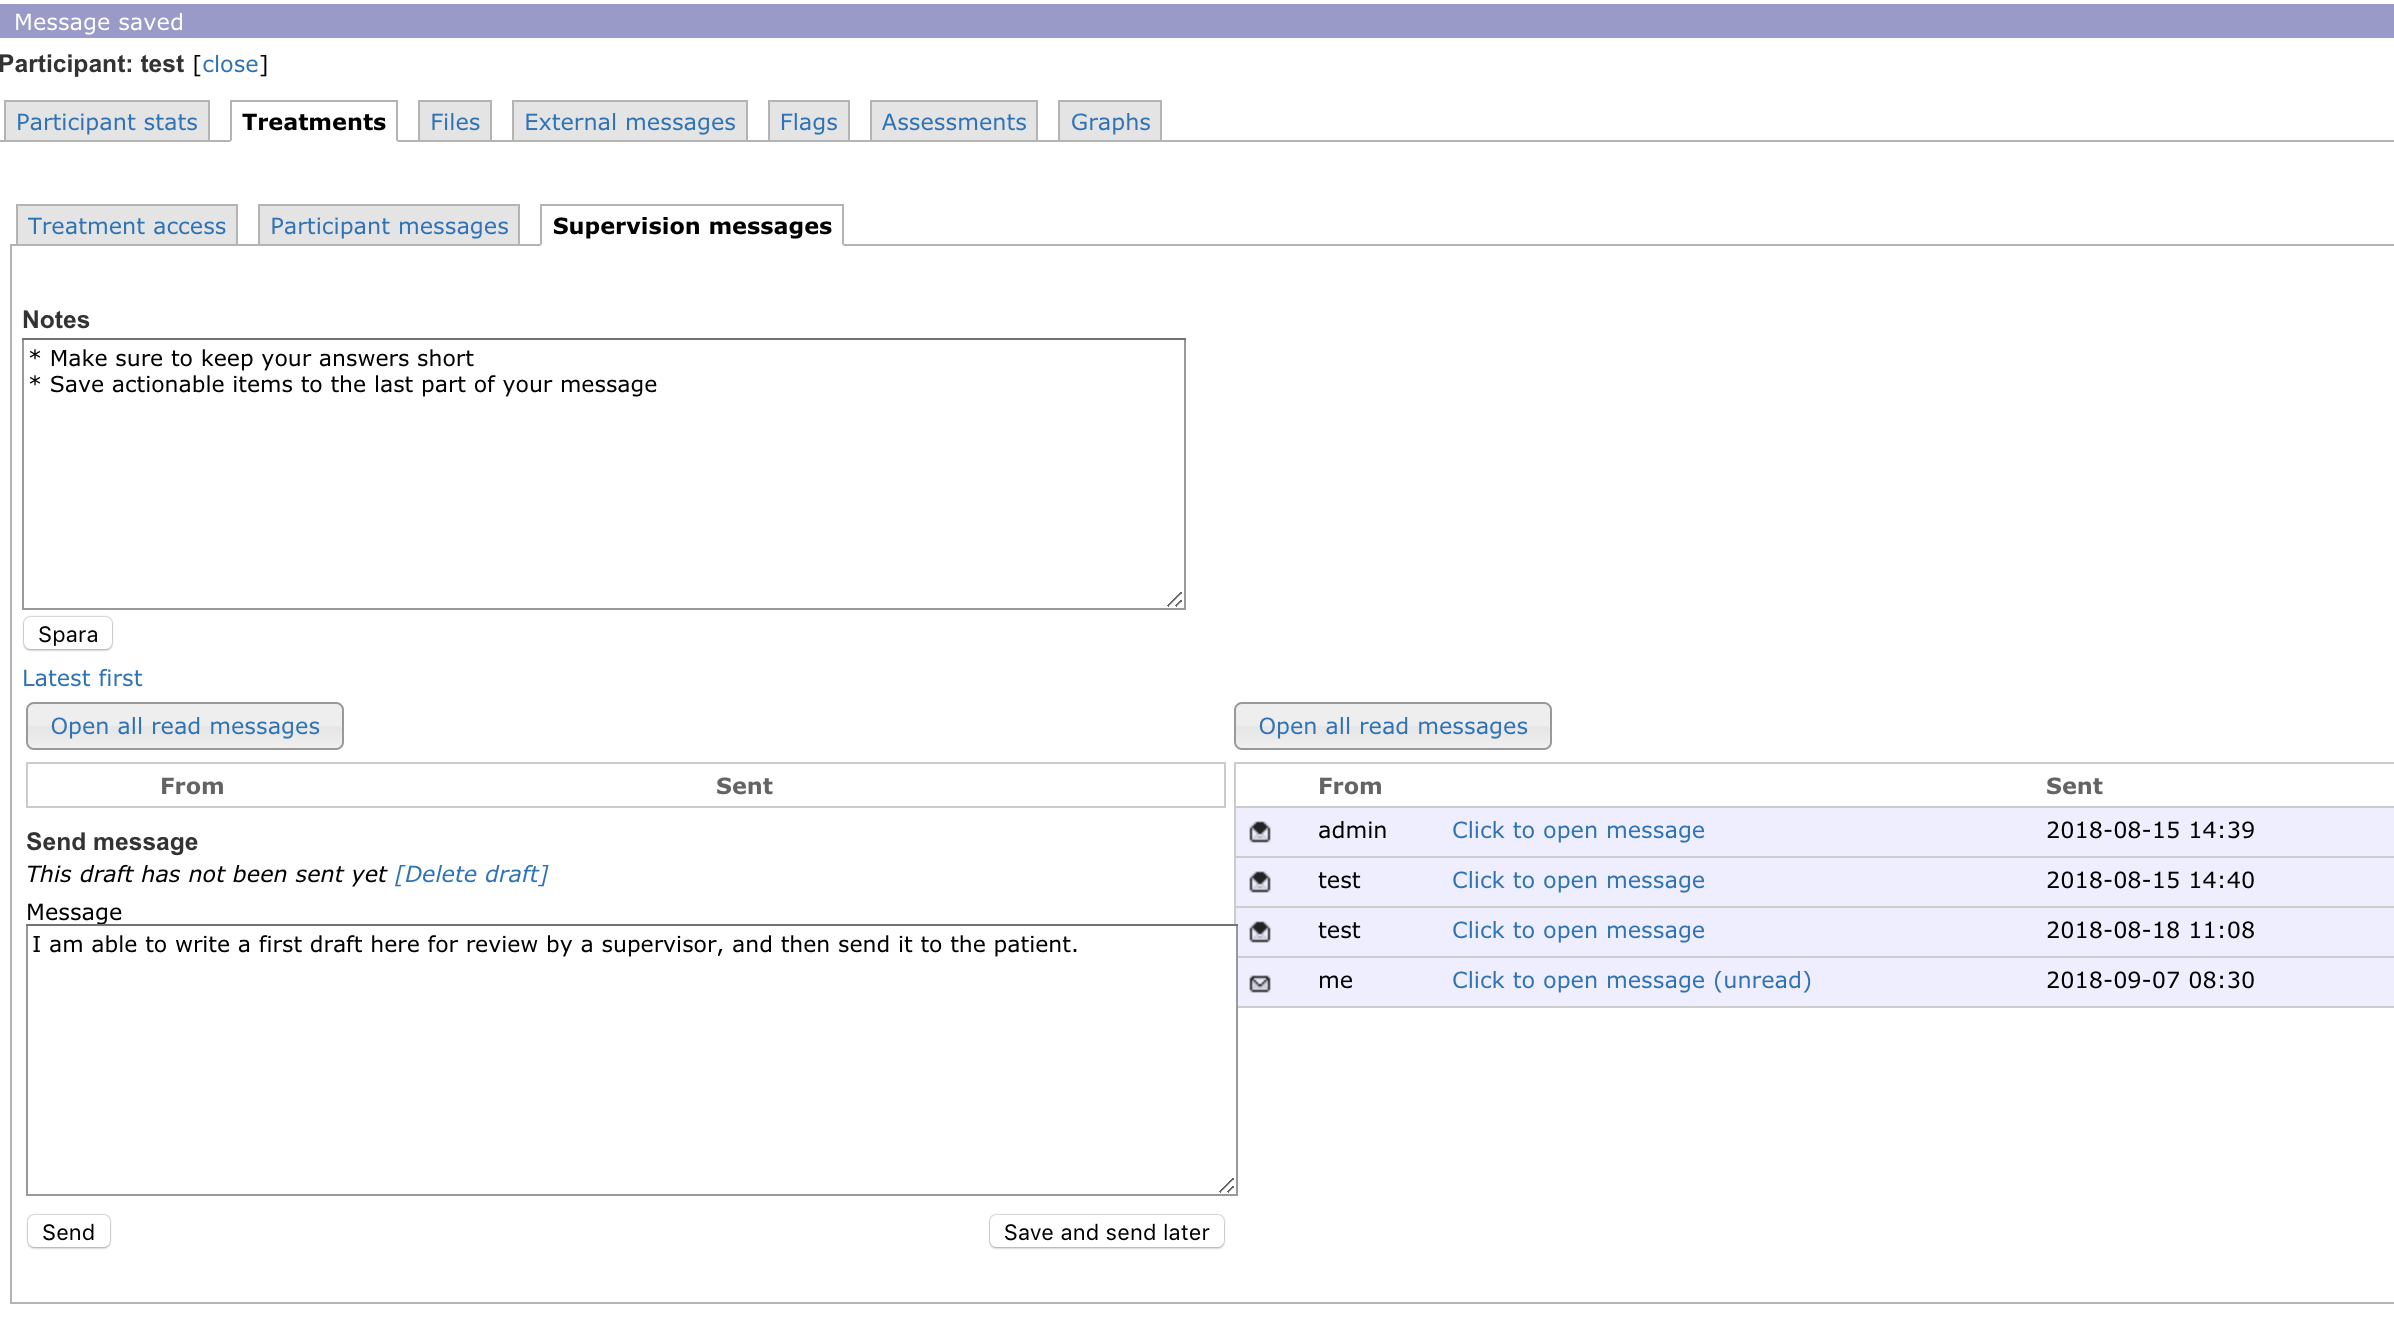
\includegraphics{images/supervision.png}

\hypertarget{assign-new-therapist}{%
\section{Assign new therapist}\label{assign-new-therapist}}

The most typical scenario is that each patient is treated by one
therapist throughout treatment, but it is not uncommon for a second
therapist to act as backup if the primary therapist is not available.

To assign another therapist or change therapist, navigate to the patient
in question and click the \emph{Participant stats} tab. At the bottom of
that page, there is a list of therapists and those assigned to the
patient will have a checkmark next to them. Simply un-check whoever is
to be removed and check whoever is to be assigned the patient.

\begin{figure}
\centering
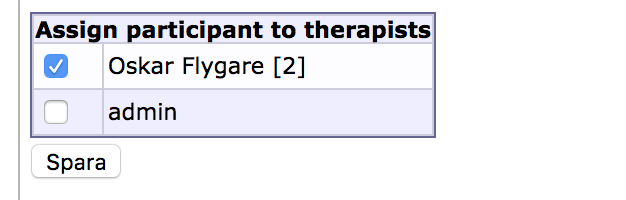
\includegraphics{images/assign-therapist.png}
\caption{The number 2 next to Oskar Flygare indicates that he is
assigned to 2 patients}
\end{figure}

\hypertarget{create-new-patient-login}{%
\section{Create new patient login}\label{create-new-patient-login}}

To create a new patient login on the platform, go to the participant
overview by selecting \emph{Participant search} in the left-hand menu.
Select \emph{Create new participant} at the bottom of the participant
list.

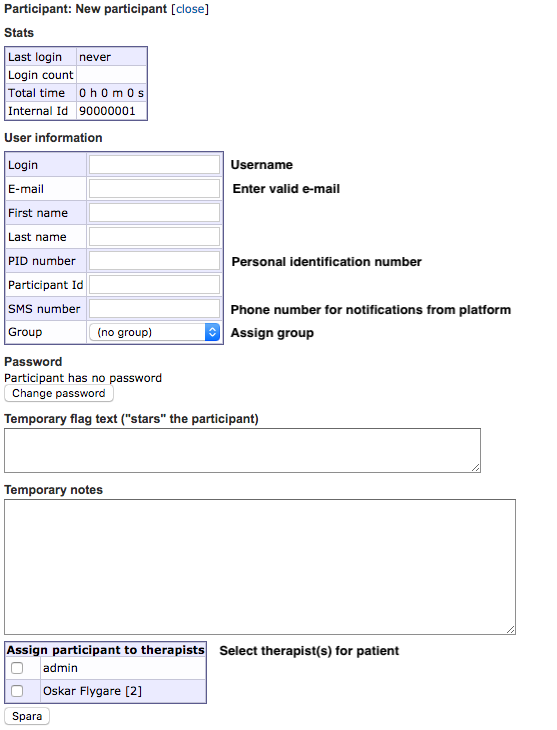
\includegraphics{images/new-participant.png}

Fields not needed are:

\begin{itemize}
\tightlist
\item
  Participant ID: Internal ID for the platform. Usually not needed.
\item
  Password: New patient logins are created without passwords. The first
  time the patient logs onto the platform they will be asked to generate
  a password
\item
  Temporary flag text: Usually not needed at creation but might come in
  handy later for communicating between therapists
\item
  Temporary notes: Usually not needed
\end{itemize}

\hypertarget{ocd-net-and-bdd-net-for-patients}{%
\section{OCD-NET and BDD-NET for
patients}\label{ocd-net-and-bdd-net-for-patients}}

We encourage therapists using OCD-NET and BDD-NET to login with one of
the test patient accounts to see what the platform looks like for
patients. See below for a quick overview of the registration process.

\hypertarget{access}{%
\subsection{Access}\label{access}}

\hypertarget{registration}{%
\subsection{Registration}\label{registration}}

\hypertarget{information-for-patients}{%
\subsection{Information for patients}\label{information-for-patients}}

\hypertarget{using-the-technology-as-a-patient}{%
\subsection{Using the technology as a
patient}\label{using-the-technology-as-a-patient}}

\hypertarget{ocd-net-therapist-manual}{%
\chapter{OCD-NET therapist manual}\label{ocd-net-therapist-manual}}

\hypertarget{what-is-ocd-net}{%
\section{What is OCD-NET?}\label{what-is-ocd-net}}

The treatment in OCD-NET is based on established treatment protocols for
OCD \citep{foa2012}, and focuses on exposure with response prevention
(ERP). This means patients do most of the active treatment work away
from their computer or mobile device, for example when they are
performing exposure and response prevention exercises.

\hypertarget{who-is-suitable-for-ocd-net}{%
\subsection{Who is suitable for
OCD-NET}\label{who-is-suitable-for-ocd-net}}

OCD-NET has been developed to treat adult patients with OCD. In previous
trials evaluating OCD-NET, participants have had comorbid conditions
such as depression and anxiety, while autism spectrum disorder,
psychotic symptoms and substance use disorder have been exclusion
criteria.

The intended use of OCD-NET is within a stepped-care model where
patients are offered low-intensity treatments as a first step,
\href{https://www.nice.org.uk/guidance/CG31/chapter/1-Guidance\#stepped-care-for-adults-young-people-and-children-with-ocd-or-bdd}{see
the NICE-guidelines}. We therefore recommend that OCD-NET is primarily
used for patients with mild to moderate symptom severity without
comorbid autism spectrum disorder, psychotic symptoms, or substance use
disorder.

\hypertarget{presenting-ocd-net-as-an-option-to-the-patient}{%
\subsection{Presenting OCD-NET as an option to the
patient}\label{presenting-ocd-net-as-an-option-to-the-patient}}

It is important to stress that previous trials of OCD-NET have been
conducted on patients that have actively requested internet-based
treatment when giving this option. Thus, forcing someone to undertake a
treatment they do not agree with is unhelpful at the very least and can
also be harmful.

With that in mind, we believe there are two particularly strong
arguments for the use of OCD-NET rather than face-to-face therapy:
patients can access the treatment content and therapist therapist
support whenever they want to, and treatment can start right away rather
than after a waiting time.

We have also found that many patients like to contribute to research and
the development of new treatments. For example, most patients will see
the benefit of evaluating remote treatment options.

Other suggestions:

\begin{itemize}
\tightlist
\item
  Write your first message on the first day of treatment to welcome the
  patient and notify them of ways to contact you with questions
\item
  Provide encouragement throughout treatment to motivate the patient and
  establish a therapeutic working alliance
\end{itemize}

\hypertarget{modules-in-ocd-net}{%
\subsection{Modules in OCD-NET}\label{modules-in-ocd-net}}

There are 10 modules in OCD-NET, which patients are expected to complete
in 12 weeks. Each module consists of texts and uses well established
evidence based interventions for OCD, with exposure and response
prevention (ERP) being the core intervention. To progress to the next
module participants have to complete homework assignments (such as
reading text material, answering a quiz at the end of each module,
completing worksheets, or report about ERP exercises) which are viewed
by their therapist.

\begin{longtable}[]{@{}ll@{}}
\toprule
\begin{minipage}[b]{0.47\columnwidth}\raggedright
\textbf{Treatment module}\strut
\end{minipage} & \begin{minipage}[b]{0.47\columnwidth}\raggedright
\textbf{Content}\strut
\end{minipage}\tabularnewline
\midrule
\endhead
\begin{minipage}[t]{0.47\columnwidth}\raggedright
1. Introduction to the treatment\strut
\end{minipage} & \begin{minipage}[t]{0.47\columnwidth}\raggedright
Introduction to CBT Information about OCD\strut
\end{minipage}\tabularnewline
\begin{minipage}[t]{0.47\columnwidth}\raggedright
2. A CBT model of OCD\strut
\end{minipage} & \begin{minipage}[t]{0.47\columnwidth}\raggedright
Psychological model of OCD with patient examples\strut
\end{minipage}\tabularnewline
\begin{minipage}[t]{0.47\columnwidth}\raggedright
3. Thinking mistakes in OCD\strut
\end{minipage} & \begin{minipage}[t]{0.47\columnwidth}\raggedright
Common cognitive biases and unhelpful interpretations of thoughts in
OCD\strut
\end{minipage}\tabularnewline
\begin{minipage}[t]{0.47\columnwidth}\raggedright
4. Introduction to ERP\strut
\end{minipage} & \begin{minipage}[t]{0.47\columnwidth}\raggedright
Goal setting Planning ERP exercises\strut
\end{minipage}\tabularnewline
\begin{minipage}[t]{0.47\columnwidth}\raggedright
5. More about ERP\strut
\end{minipage} & \begin{minipage}[t]{0.47\columnwidth}\raggedright
Best practices in ERP\strut
\end{minipage}\tabularnewline
\begin{minipage}[t]{0.47\columnwidth}\raggedright
6. Imaginal exposure\strut
\end{minipage} & \begin{minipage}[t]{0.47\columnwidth}\raggedright
Instructions to get started with imaginal exposures\strut
\end{minipage}\tabularnewline
\begin{minipage}[t]{0.47\columnwidth}\raggedright
7. Re-exposure\strut
\end{minipage} & \begin{minipage}[t]{0.47\columnwidth}\raggedright
Undoing habitual compulsions\strut
\end{minipage}\tabularnewline
\begin{minipage}[t]{0.47\columnwidth}\raggedright
8. Difficulties during treatment\strut
\end{minipage} & \begin{minipage}[t]{0.47\columnwidth}\raggedright
Common problems in ERP Motivation traps\strut
\end{minipage}\tabularnewline
\begin{minipage}[t]{0.47\columnwidth}\raggedright
9. Long term goals and values\strut
\end{minipage} & \begin{minipage}[t]{0.47\columnwidth}\raggedright
Increasing valued behaviours Aligning ERP exercises with long term
values\strut
\end{minipage}\tabularnewline
\begin{minipage}[t]{0.47\columnwidth}\raggedright
10. Summary and wrap up\strut
\end{minipage} & \begin{minipage}[t]{0.47\columnwidth}\raggedright
Maintaining progress Relapse prevention\strut
\end{minipage}\tabularnewline
\bottomrule
\end{longtable}

We view modules 1, 2, 4, and 5 as the core modules in OCD-NET. Modules 1
and 2 consist of two essential features: the patient needs to report at
least some intrusions/compulsions in the OCD diary, and the patient
needs to understand the CBT model of OCD. These two features are the
building blocks for the subsequent ERP exercises in module 4 and 5. We
usually recommend patients to do modules 1-5 in a relatively quick pace
in order to get to the active treatment as soon as possible. It is not
crucial to have a detailed plan for each ERP exercise before starting;
you should encourage patients to get started and fine-tune ERP exercises
as they go along.

You can consider modules 3 and 6 as optional for the patient. We advise
all our patients to read the text in module 3 (thinking mistakes), but
if the patient does not feel that this cognitive intervention is
relevant for them, we proceed directly to module 4 (ERP). Module 6
(imaginal exposure) may be beneficial for some patients but our
experience is that many patients skip this intervention. Although the
text is written from a habituation lens, we often tell our patients that
imaginal exposure may be a tool to learn that having a thought or image
is not the same as acting that way, and to tolerate uncertainty.

The number of completed modules is not an essential predictor of
treatment outcomes in OCD-NET. We have two goals only: get the patient
to module 5 and get the patient to do a lot of ERP exercises. Thus it is
not essential that the patient progress through all modules as long as
he/she does ERP and reports this frequently to the therapist. Patients
will gain access to all modules at the end of treatment, and will be
able to log onto the platform for one year after completing the OCD-NET
treatment. Thus, the role of the therapist is to encourage the patient
to do ERP exercises and help them to design and evaluate ERP exercises
effectively.

Modules 6-9 can be opened in any order to fit the needs of each patient.
For example, a patient might not have any use of imaginal exposure but
finds that they have a hard time refraining from habitual compulsions.
In that case, you may open up module 7 (re-exposure) instead of module 6
(imaginal exposure). Other patients may struggle with ERP exercises and
will find module 8 (difficulties during the treatment) useful. Use your
clinical intuition.

\hypertarget{closing-remarks}{%
\section{Closing remarks}\label{closing-remarks}}

We hope that you have found this therapist guide useful. Our goal has
been to present a few ideas about how to deliver OCD-NET effectively.
These are just the first building blocks and you will likely find that
adaptations are needed to your particular patients and your own style as
a therapist.

We strive to continuously update and improve this material and would
appreciate any feedback. You can reach us at
\href{mailto:ocdnet.support@webcbt.se}{\nolinkurl{ocdnet.support@webcbt.se}}
or talk to us in person at a training session.

\hypertarget{bdd-net-therapist-manual}{%
\chapter{BDD-NET therapist manual}\label{bdd-net-therapist-manual}}

\hypertarget{what-is-bdd-net}{%
\section{What is BDD-NET?}\label{what-is-bdd-net}}

BDD-NET consists of eight interactive modules and focuses on exposure
with response prevention (ERP). This means that patients do most of the
active treatment work away from their computer or mobile device, for
example when they are performing ERP exercises.

\hypertarget{who-is-suitable-for-bdd-net}{%
\section{Who is suitable for
BDD-NET}\label{who-is-suitable-for-bdd-net}}

BDD-NET is developed to treat adults with body dysmorphic disorder
(BDD). Patients may have comorbid conditions, for example other anxiety
disorders, depression, or OCD. Patients may also take antidepressant
medication during the course of treatment. We recommend that patients do
not change the dose during the course of treatment. BDD-NET may also be
delivered to patients with any level of BDD symptom severity.

Contraindications include having a personality disorder that might
interfere with treatment (such as borderline personality disorder),
psychotic symptoms, an ongoing substance abuse, or acute suicidal
ideation. BDD-NET is text-based and so requires sufficient reading
skills and understanding of English. We recommend that the patient is
referred to face-to-face treatments if contraindications are discovered.

\hypertarget{presenting-bdd-net-as-an-option-to-the-patient}{%
\section{Presenting BDD-NET as an option to the
patient}\label{presenting-bdd-net-as-an-option-to-the-patient}}

\hypertarget{assessing-insight}{%
\subsection{Assessing insight}\label{assessing-insight}}

Participating in internet-based treatments such as BDD-NET is voluntary,
and therapists need to make sure that patients are willing to challenge
their BDD in treatment. Lack of insight is common in BDD and BDD-NET is
designed to work for patients that express varying degrees of insight.
It is our experience that patients need to at least be willing to try
out alternative behaviours during the course of treatment, even if they
might still be convinced that their appearance concerns are justified at
the start of treatment.

\hypertarget{managing-expectations}{%
\subsection{Managing expectations}\label{managing-expectations}}

Some patients may have expectations to be completely free from anxiety
after BDD-NET, and that all that is required of them is to read and
understand what is written in the treatment modules. Such expectations
are discussed in module 4 (goal setting) but therapists are advised to
assess whether patients are willing to challenge their BDD through
exposure with response prevention and try out alternative behaviours
before starting BDD-NET. If someone completely refuses to try new
behaviours they are unlikely to participate in BDD-NET fully and benefit
from the treatment.

\hypertarget{a-good-start-in-bdd-net}{%
\subsection{A good start in BDD-NET}\label{a-good-start-in-bdd-net}}

Many patients with BDD find BDD-NET an interesting treatment option,
particularly those who avoid many activities due to their appearance
concerns. The strongest arguments in favour of ICBT treatments like
BDD-NET, from a patient perspective, is that the treatment content and
the therapist are accessible throughout the week, and that the treatment
starts promptly after evaluation rather than after a time in waiting
list.

To give patients a positive first impression of the treatment, we
suggest that therapists write their first message on the first day of
treatment to welcome the patient and notify them of ways to contact you.
Provide encouragement throughout treatment to motivate the patient and
establish a therapeutic working alliance. Patients sometimes struggle
with crucial treatment components such as the BDD diary exposure with
response prevention (ERP), so make sure to provide extra support if
patients get stuck at those points.

\hypertarget{modules-in-bdd-net}{%
\section{Modules in BDD-NET}\label{modules-in-bdd-net}}

Below is an overview of the eight treatment modules. We recommend that
you look at them from a patient's point of view before starting the
first treatment.

\begin{longtable}[]{@{}ll@{}}
\toprule
\begin{minipage}[b]{0.47\columnwidth}\raggedright
\textbf{Treatment module}\strut
\end{minipage} & \begin{minipage}[b]{0.47\columnwidth}\raggedright
\textbf{Content}\strut
\end{minipage}\tabularnewline
\midrule
\endhead
\begin{minipage}[t]{0.47\columnwidth}\raggedright
1. Introduction to BDD and the treatment\strut
\end{minipage} & \begin{minipage}[t]{0.47\columnwidth}\raggedright
An introduction to BDD Introduction to the treatment content\strut
\end{minipage}\tabularnewline
\begin{minipage}[t]{0.47\columnwidth}\raggedright
2. A CBT model of BDD\strut
\end{minipage} & \begin{minipage}[t]{0.47\columnwidth}\raggedright
Psychological explanation of the link between thoughts, emotions, and
behaviours\strut
\end{minipage}\tabularnewline
\begin{minipage}[t]{0.47\columnwidth}\raggedright
3. Interpretation traps\strut
\end{minipage} & \begin{minipage}[t]{0.47\columnwidth}\raggedright
Common cognitive biases in BDD\strut
\end{minipage}\tabularnewline
\begin{minipage}[t]{0.47\columnwidth}\raggedright
4. Introduction to ERP\strut
\end{minipage} & \begin{minipage}[t]{0.47\columnwidth}\raggedright
Goal setting and planning of exposure with response prevention\strut
\end{minipage}\tabularnewline
\begin{minipage}[t]{0.47\columnwidth}\raggedright
5. More about ERP\strut
\end{minipage} & \begin{minipage}[t]{0.47\columnwidth}\raggedright
Doing and evaluating exposure with response prevention exercises\strut
\end{minipage}\tabularnewline
\begin{minipage}[t]{0.47\columnwidth}\raggedright
6. Values and Goals\strut
\end{minipage} & \begin{minipage}[t]{0.47\columnwidth}\raggedright
Identifying and acting in accordance with personal values\strut
\end{minipage}\tabularnewline
\begin{minipage}[t]{0.47\columnwidth}\raggedright
7. Difficulties during treatment\strut
\end{minipage} & \begin{minipage}[t]{0.47\columnwidth}\raggedright
Strategies to deal with common difficulties and setbacks\strut
\end{minipage}\tabularnewline
\begin{minipage}[t]{0.47\columnwidth}\raggedright
8. Summary and Relapse Prevention\strut
\end{minipage} & \begin{minipage}[t]{0.47\columnwidth}\raggedright
Treatment summary, evaluation of treatment, and designing a relapse
prevention plan\strut
\end{minipage}\tabularnewline
\bottomrule
\end{longtable}

As you can see, the emphasis is on doing exposure with response
prevention (ERP), which we view as the main component of BDD-NET. You
typically want to encourage the patient to progress through the first
three modules as fast as possible, check that they have understood the
rationale for ERP, and then start doing ERP. Once a patient is doing
regular ERP-exercises, you can open up modules 6-7 for them to complete
while continuing to do daily ERP. Module 8 can then be opened up with
one to two weeks left in treatment.

\hypertarget{closing-remarks-1}{%
\section{Closing remarks}\label{closing-remarks-1}}

The strategies outlined here should be viewed as the first building
blocks in becoming an effective ICBT therapist using BDD-NET. As in
regular clinical practice, we recommend continuous supervision and that
therapists discuss difficult cases with colleagues.

We strive to continuously update and improve this material and would
appreciate any feedback. You can reach us at
\href{mailto:ocdnet.support@webcbt.se}{\nolinkurl{ocdnet.support@webcbt.se}}
or talk to us in person at a training session.

\hypertarget{being-an-effective-icbt-therapist}{%
\chapter{Being an effective ICBT
therapist}\label{being-an-effective-icbt-therapist}}

Being a therapist in internet-based CBT (ICBT) differs in several ways
from regular face-to-face treatment. The first difference is the mode of
communication: asynchronous text messages rather than live face-to-face
talking. The second is that therapists are more closely integrated in
the treatment content, and will rely more heavily on the written
material. Third, there is less therapist oversight during active ERP
exercises. We will discuss these implications below.

\hypertarget{keep-your-messages-short}{%
\section{Keep your messages short}\label{keep-your-messages-short}}

Messages should be concise and to the point but still using a personal
touch. The main aim is to provide encouragement and reinforce key
behaviours in the treatment, such as registrations in the OCD/BDD diary
and performing ERP exercises.

There are some exceptions to this rule. Therapists are advised to write
longer messages when needed: to highlight examples in the diary that are
informative and relate these to the CBT model of OCD/BDD, or to provide
encouragement by linking ERP exercises to a patient's long-term goals
and values.

\hypertarget{write-often}{%
\section{Write often}\label{write-often}}

Frequent communication is particularly useful at the start of treatment
and when patients are in the startup phase of ERP. In many ways, ICBT
may be an even more intensive treatment than traditional face-to-face
CBT for patients. Our standard procedure is to contact patients at least
twice weekly, but more often when needed. For example, therapists may
confirm an exposure exercise in the morning and check in during the
afternoon for a follow-up.

There are exceptions to the rule of frequent messages: some patients
will prefer to do ERP exercises on their own and will not have many
questions. This is perfectly fine; some patients benefit greatly from
the ICBT treatment without the therapist support.

\hypertarget{therapists-and-the-rest-of-the-content-in-icbt}{%
\section{Therapists and the rest of the content in
ICBT}\label{therapists-and-the-rest-of-the-content-in-icbt}}

As previously mentioned, ICBT is in many ways a high intensity
treatment. Patients not only respond to messages but also read module
texts, answer homework questions and questionnaires, and fill in
worksheets. The treatment becomes particularly intensive once patients
start performing daily ERP exercises. Thus, what might feel like a
low-intensity treatment from the therapist perspective is actually be
very intensive for patients.

Therapists should keep in mind that patients do many other things
besides writing and responding to messages. Corrective feedback is
sometimes necessary in order to design, do, and evaluate effective ERP
exercises. We recommend that therapists are generally restrictive about
corrective feedback when it is not clearly needed for ERP, but
therapists should use their clinical judgment in these situations.

\hypertarget{promoting-hands-on-erp-exercises}{%
\section{Promoting hands-on ERP
exercises}\label{promoting-hands-on-erp-exercises}}

With the restrictions on therapist input in ICBT, what therapists attend
to in messages signal what patients are expected to work on during
treatment. A typical message from a patient mid-treatment might include
a summary of their latest ERP exercise, comments about what they have
found challenging, and a couple of questions about the treatment
content. It is very tempting to try to answer the questions and make
suggestions for how to deal with the challenges in the response, but
that could shift attention away from doing ERP exercises. Rather, we
want to encourage the patient to continue doing ERP because that is the
key behaviour for them to get better in the long-term.

Therapists should therefore strive to balance feedback to aid
understanding with actionable advice that patients can put into
practice. For example, a lack of clarity in an ERP exercise or choosing
the wrong ERP exercise could result in the patient getting stuck and
asking questions. A therapist could then address both the uncertainties
and promote behaviour change through ERP by suggesting a variation of
the ERP exercise or suggesting a new one that is better suited for the
situation. This is likely to be a more effective strategy compared to
just addressing the questions one by one without linking them to ERP
exercises or behaviour change.

\hypertarget{lack-of-therapist-guided-exposure-exercises}{%
\section{Lack of therapist-guided exposure
exercises}\label{lack-of-therapist-guided-exposure-exercises}}

We do not have the privilege of guiding patients through ERP exercises
in ICBT. This means that therapists will have to focus on the essentials
when giving corrective feedback to patients. Correcting every little
detail before each exercise will in this context probably be
counter-productive and might in fact confuse the patient. Instead, our
focus is to get patients going with the ERP exercises. Wrinkles can be
ironed out along the way.

\hypertarget{dealing-with-patients-with-low-engagement}{%
\section{Dealing with patients with low
engagement}\label{dealing-with-patients-with-low-engagement}}

The best way to deal with low engagement is to prevent it from happening
to begin with. Strategies to prevent low engagement include:

\begin{enumerate}
\def\labelenumi{\arabic{enumi}.}
\tightlist
\item
  Writing frequently (especially in the beginning of treatment in order
  to keep up momentum)
\item
  Focusing on encouragement in written messages
\item
  Promptly calling patients that do not respond to messages
\item
  Providing support and help to patients that struggle with ERP
  exercises
\end{enumerate}

If a patient becomes less active on the treatment platform, it does not
necessarily mean that they have stopped working with the treatment or
have given up on the treatment. Some inactive patients are doing a lot
of treatment work in their daily life but do not report this
spontaneously to their therapist.

\hypertarget{strategies-when-patients-express-lack-of-time-to-work-on-the-treatment}{%
\subsection{Strategies when patients express lack of time to work on the
treatment}\label{strategies-when-patients-express-lack-of-time-to-work-on-the-treatment}}

One common reason for low engagement is that the patient struggles to
find the time to work on ICBT. We recommend that therapists encourage
any small steps the patient takes and that they prioritise ERP exercises
away from the computer over reading additional modules.

If a patient is completely unable to work on the treatment right now,
ask him/her if it possible to delay the start of treatment. The absolute
majority of patients responding to OCD-NET and BDD-NET experience this
gain within the first 5 weeks after starting treatment. Thus, even if
the patient is delayed and start the treatment at week 5, it is still
possible to achieve a significant improvement given that the patient
works with the treatment intensively.

\hypertarget{strategies-when-patients-express-skepticism-about-icbt}{%
\subsection{Strategies when patients express skepticism about
ICBT}\label{strategies-when-patients-express-skepticism-about-icbt}}

Some patients may be skeptical about ICBT in general or in their ability
to complete a remote treatment without face-to-face support from a
therapist. We recommend that therapists validate and acknowledge that
these concerns are common early in treatment and, importantly, help
skeptical patients experience \emph{early wins} by starting with swift
and easy ERP exercises.

It is important to stress that OCD-NET and BDD-NET have never been
designed as full alternatives to face-to-face CBT but should instead be
seen as a complementary approach. Patients who are skeptical about ICBT
from the beginning will probably not benefit from this treatment
modality. Alternative formats and treatments are probably a more
feasible option in these cases.

\hypertarget{technical-support}{%
\chapter{Technical support}\label{technical-support}}

This page contains support for common issues that might arise when using
the OCD-NET and BDD-NET treatments.

\hypertarget{technical-support-for-patients}{%
\section{Technical support for
patients}\label{technical-support-for-patients}}

The platform is designed to be user-friendly for patients with varying
technical know-how. They will, however, require technical support from
time to time. If patients report technical issues that you cannot
address yourself, send an email to
\href{mailto:ocdnet.support@webcbt.se}{\nolinkurl{ocdnet.support@webcbt.se}}
and ask for assistance.

\hypertarget{forgotten-username-or-password}{%
\subsection{Forgotten username or
password}\label{forgotten-username-or-password}}

If a patient has forgotten their password, they can request a new one at
the login screen:

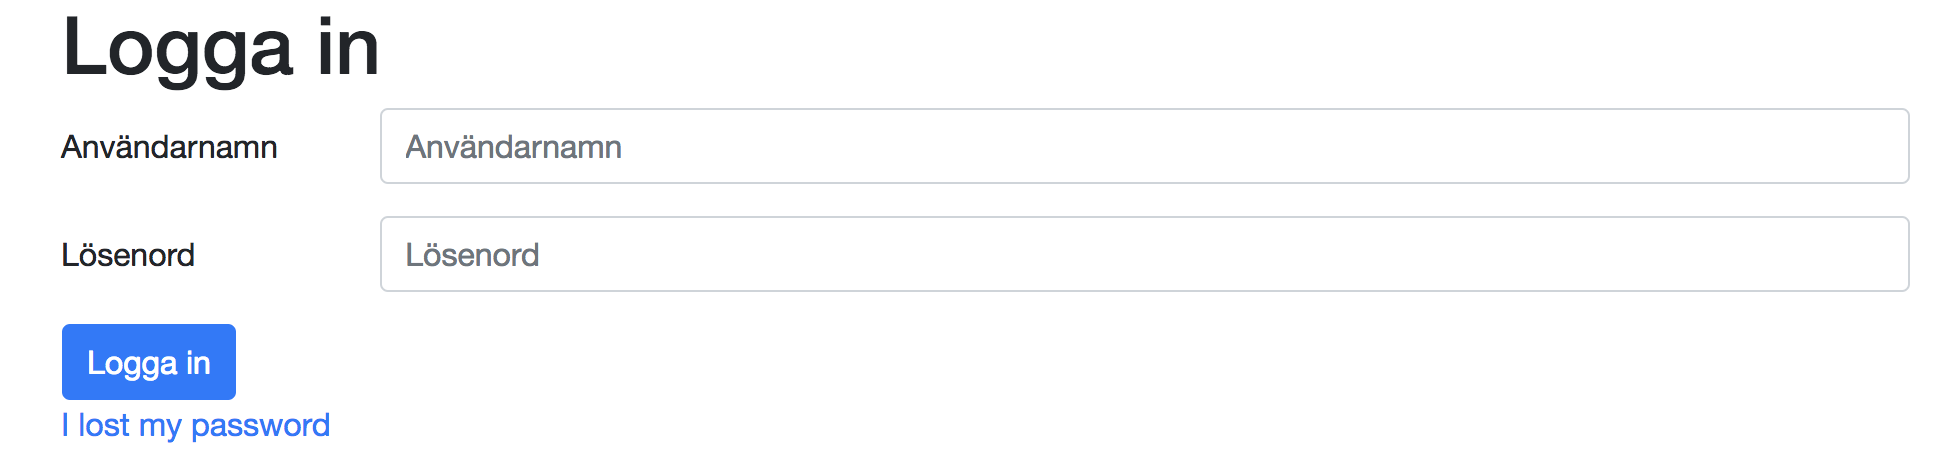
\includegraphics{images/patient-lost-password.png}

If they have forgotten their username, simply look at their
\emph{Participant stats} and \textbf{Login} is their username.

If a patient is unable to generate a new password on their own, navigate
to the patient in question and the \emph{Participant stats} tab. Click
the \emph{Change password} button. The site generates a new, secure,
password that can be sent to the patient via SMS.

\begin{figure}
\centering
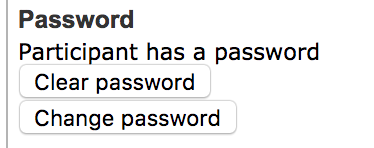
\includegraphics{images/change-password.png}
\caption{Change password button}
\end{figure}

\hypertarget{the-website-does-not-work}{%
\subsection{The website does not work}\label{the-website-does-not-work}}

This is usually for one of three reasons: wrong information
(URL/username/password), the patient is using an out of date web
browser, or there is an issue with cookies on the site.

\hypertarget{wrong-urlusernamepassword}{%
\subsubsection{Wrong
URL/username/password}\label{wrong-urlusernamepassword}}

Make sure that the patient has correct information for all three. Also
make sure that there are no errors in the username!

\begin{itemize}
\tightlist
\item
  URL is \url{webcbt.se/ocdnet} for OCD and \url{webcbt.se/bddnet} for
  BDD
\item
  Username is indicated by ``Login'' at \emph{Participant stats}
\item
  Their password is hidden to therapists and can be re-generated by
  patients themselves or by therapists (see above)
\end{itemize}

\hypertarget{recommended-web-browsers}{%
\subsubsection{Recommended web
browsers}\label{recommended-web-browsers}}

The treatment is accessible for both desktop web browsers and mobile web
browsers (iOS, Android). The platform works best for either
\textbf{Google Chrome}, \textbf{Firefox}, or \textbf{Safari}. Internet
explorer and Microsoft Edge are not recommended, although newer versions
of those browsers usually work just fine.

\hypertarget{cookies-and-cache}{%
\subsubsection{Cookies and cache}\label{cookies-and-cache}}

Sometimes the browser will save cookies that interfere with access to
the treatment platform. This can usually be resolved by clearing cookies
and restarting the browser.

\begin{itemize}
\tightlist
\item
  \href{https://support.google.com/chrome/answer/95647?co=GENIE.Platform\%3DDesktop\&hl=en}{Google
  Chrome}
\item
  \href{https://support.mozilla.org/en-US/kb/delete-cookies-remove-info-websites-stored}{Firefox}
\item
  \href{https://support.apple.com/kb/ph21411?locale=en_US}{Safari
  desktop}
\item
  \href{https://support.apple.com/en-gb/HT201265}{Safari iOS}
\end{itemize}

\hypertarget{technical-support-for-therapists}{%
\section{Technical support for
therapists}\label{technical-support-for-therapists}}

\hypertarget{creating-an-account}{%
\subsection{Creating an account}\label{creating-an-account}}

Send an e-mail to us
\href{mailto:ocdnet.support@webcbt.se}{\nolinkurl{ocdnet.support@webcbt.se}}
containing the following information:

\begin{itemize}
\tightlist
\item
  Username
\item
  Full name
\item
  e-mail
\item
  Phone number (to receive login codes via text messages)
\end{itemize}

We then create a user and generate a password to be replaced at the
first login.

\hypertarget{forgotten-password}{%
\subsection{Forgotten password}\label{forgotten-password}}

Admins are able to reset therapist passwords in the \emph{Therapist} tab
of the left-hand menu. Click the button called ``Must change password''
to initiate a password change for that user.

\hypertarget{other-technical-issues}{%
\section{Other technical issues}\label{other-technical-issues}}

Have you spotted an error in the treatment content? Are the
questionnaires not displaying correctly? Did you accidentally make some
changes that you are not able to revert?

Anything else that is not reviewed in this guide, please let ut know by
sending an e-mail to us at
\href{mailto:ocdnet.support@webcbt.se}{\nolinkurl{ocdnet.support@webcbt.se}}
and we will help you.

We strive to improve the treatment content and the experience for
therapists continuously and welcome any feedback!

\hypertarget{references}{%
\chapter{References}\label{references}}

\bibliography{bibliography.bib,packages.bib}


\end{document}
